\documentclass[a4paper, 11pt, oneside]{report} 
\usepackage[utf8]{inputenc}
\usepackage[dutch]{babel}
\usepackage{amsmath}
\usepackage{amsfonts}
\usepackage{amssymb}
\usepackage{graphicx}
\usepackage{caption}
\usepackage[table,xcdraw]{xcolor}
\usepackage[toc,page]{appendix}
\usepackage{hyperref}
\usepackage{titlesec}
\usepackage{listings}
\usepackage{float}
\usepackage{tikz}
\usetikzlibrary{trees}
\usepackage{tikz-qtree}
\usepackage{graphicx}
\usepackage{fancyref}
\usepackage{wrapfig}
\usepackage{url}
\usepackage{pdflscape}
\usepackage{fancyvrb}
\usepackage{fancyhdr}
\graphicspath{ {Afbeeldingen/} }
\usepackage{subfig}
\usepackage{tabularx}
\usepackage{apacite}
\usepackage{longtable}
\usepackage{titlecaps}
%\usepackage[T1]{fontenc}
\usepackage{titlesec, blindtext, color}
\definecolor{gray75}{gray}{0.75}
\newcommand{\hsp}{\hspace{20pt}}
\usepackage{pdfpages}


\newcolumntype{L}[1]{>{\raggedright\arraybackslash}p{#1}}

\titleformat{\chapter}[hang]{\huge\bfseries}{\thechapter\hsp\textcolor{gray75}{|}\hsp}{0pt}{\Large\bfseries}

\def\figureautorefname{Figuur}
\def\sectionautorefname{Paragraaf}
\def\chapterautorefname{Hoofdstuk}
\def\tableautorefname{Tabel}
\DeclareRobustCommand{\VAN}[3]{#2} % set up for citation

%% Sets page size and margins 
\usepackage[a4paper,top=3cm,bottom=3cm,left=3cm,right=3cm,marginparwidth=1.75cm]{geometry}

\author{M.W.J. Berentsen}
\font\myfont=cmr12 at 40pt
\title{\myfont Drone meshnetwerk simulatie}
\usepackage{titling}

\newcommand{\subtitle}[8]{%
	\posttitle{%
		\par\end{center}
	\begin{center}\large#1\end{center}
	\vskip0.5em
	\begin{center}\large#2\end{center}
	\begin{center}\large#3\end{center}
	\begin{center}\large#4\end{center}
    \begin{center}\large#5\end{center}
    \begin{center}\large#6\end{center}
    \begin{center}\large#7\end{center}
    \begin{center}\large#8\end{center}
	\vskip0.5em}%
}

\subtitle{Software Requirements Specification}{HAN Arnhem}{561399}{MWJ.Berentsen@student.han.nl}{Versie 1}{Alten Nederland B.V.}{Docent: J. Visch, MSc}{Assessor: ir. C.G.R. van Uffelen}

\setlength{\parindent}{0pt}
\setlength{\parskip}{5pt plus 2pt minus 1pt}



\hypersetup{colorlinks=true, urlcolor=red,citecolor=black,linkcolor=blue}  % Colours hyperlinks in blue, but this can be distracting if there are many links.
\setcounter{tocdepth}{2}



\begin{document}
\begin{figure}
\begin{center}
\includegraphics[scale=0.1]{alten}\end{center}
\end{figure}
\maketitle

%\section*{Voorwoord}
%\addcontentsline{toc}{section}{\protect\numberline{}Voorwoord}
%\pagebreak

%Geschikt voor minimaal 50 nodes; Kan slecht of geen signaal nabootsen

\tableofcontents
\clearpage
%\section*{Begrippenlijst}

% Please add the following required packages to your document preamble:
% \usepackage[table,xcdraw]{xcolor}
% If you use beamer only pass "xcolor=table" option, i.e. \documentclass[xcolor=table]{beamer}
%\begin{table}[H]
%\centering

%\label{begrippen}
%\begin{tabular}{|l|l|}
%\hline
%\rowcolor[HTML]{C0C0C0}
%Term        & Omschrijving                                                         \\ \hline
%term        & Omschrijving                                                      	\\ \hline

%\end{tabular}
%\caption{Begrippenlijst}
%\end{table}

%\clearpage

%\section*{Samenvatting}
%\addcontentsline{toc}{section}{\protect\numberline{}Samenvatting}
%\pagebreak


\chapter{Inleiding}
\label{inleiding}
\section{Algemene beschrijving}
\label{inleiding:beschrijving}
Het volgende verslag betreft de Software Requirements Specification voor de afstudeerstage van Maurice Berentsen (hierna: student).
Dit document volgt het document: \textit{"Software Requirements Specification Template"} \cite{template:srs}
 

\section{Doel van dit document}
\label{inleiding:doelvanditdoucment}

Het doel is dat de lezer aan het einde van dit document begrijpt hoe de functionaliteit geïmplementeerd zal worden in het op te leveren product. Het document laat zien hoe de flow van het programma loopt en welke classes in de software worden gebruikt. Een lezer van dit document zou met de juiste technische kennis de volledige applicatie moeten kunnen maken zoals het bedacht is door de ontwerper.  

\section{Actoren en hun eigenschappen}
\label{inleiding:gebruikers}
In deze paragraaf worden de actoren van het systeem omschreven. 
Elke actor wordt kort omgeschreven per sub-paragraaf 


\section{Werkomgeving}
\label{inleiding:werkomgeving}
Deze paragraaf omschrijft zowel de hardware- als softwareomgeving waarin dit project wordt uitgevoerd. 

\subsection{Arduino UNO}
\label{inleiding:werkomgeving:arduino}
De Arduino UNO is gekozen als ontwikkelbord die gebruikt wordt in het opzetten van de onderlinge communicatie.
Deze Arduino is gekozen omdat deze gemakkelijk leent voor het bouwen van prototype.
Dit doet de Arduino door zijn aanbod van 14 I/O poorten waarvan er zes bruikbaar zijn als analoge poort en het aanbieden van zowel 3.3 als 5 volt lijnen
Hierop kan de \nameref{inleiding:werkomgeving:nrf24} aangesloten worden waarna er nog genoeg poorten overblijven voor andere hardware zoals sensoren of een internetverbinding.

De aanwezigheid van een 16MHz kristaloscillator geeft de UNO de eigenschap om accuraat genoeg een verschil in tijd te schatten.
Dit belangrijk voor het systeem aangezien het beslissingen moet kunnen nemen op basis van een verstreken tijd.

De Arduino voorzien van een ATmega328P die snel genoeg is voor het doorgeven van het communicatieverkeer en het nemen van beslissingen. 
De ATmega328P heeft 32KB flash geheugen  en 1KB EEPROM beschikbaar.  

Verder is de Arduino gekozen omdat deze via een USB aansluiting makkelijk geflasht kan worden en gedeeltelijk ondersteuning heeft voor C$++$

\subsection{NRF24}
\label{inleiding:werkomgeving:nrf24}
De NRF24 is gekozen door zijn prestaties ten opzichte van afstand.
De mogelijkheid om een snelheid aan te kunnen bieden van minimaal 250 kbps op een afstand van 500 meter maakt deze module het meest geschikt voor dit project.
Daarnaast kan de NRF24 tot zes kanalen tegelijk open houden die kunnen schakelen tussen zenden en ontvangen.
De NRF24 is in staat om per payload tot 32 bytes te versturen. 
Tenslotte is de NRF24 een transciever die werkt op een voltage van 3.3 volt waarbij de I/O pinnen 5 volt tolerant zijn wat het compatibel maakt met de \nameref{inleiding:werkomgeving:arduino}.

\subsection{Drone}
\label{inleiding:werkomgeving:drone}
Hoewel in dit project drones een essentieel onderdeel zijn wordt er niet gesproken over een specifiek merk of type drone.
De reden hiervoor is omdat er geen focus ligt op een specifieke drone en de student ook niet gecertificeerd is om te vliegen met zakelijke drones.
Er zal dus gewerkt worden met gesimuleerde drones. 
Deze hebben een interface die in staat is om een drone te laten vliegen naar een specifiek coördinaat en kan de huidige locatie aangeven.

\subsection{ROS}
\label{inleiding:werkomgeving:ros}
ROS is middleware software die gebruikt wordt voor de aansturing en simulatie van robotica. 
In het geval van dit project wordt ROS gebruikt voor de communicatie naar de \nameref{inleiding:werkomgeving:drone} toe, maar ook voor het simuleren van de \nameref{inleiding:werkomgeving:nrf24} communicatie tussen de drones. 

\subsection{Gazebo}
\label{inleiding:werkomgeving:gazebo}

\href{http://gazebosim.org/}{Gazebo} is een opensource robot simulatie framework bijzonder geschikt voor het simuleren van robotica in outdoor omgevingen door de uitgebreide Physics Engine Support.
In dit project wordt momenteel geen gebruik gemaakt van de physics engine maar doordat de onderdelen als virtuele onderdelen beschikbaar zijn in gazebo kunnen ze zo aangesloten worden op een beter gesimuleerde drone.
Deze mogelijkheid was daarom ook een hoofdreden om Gazebo te gebruiken.

\section{Ontwerp en implementatie beperkingen}
\label{inleiding:ontwerpberkingen}


\section{Product Functies}
\label{inleiding:productfuncties}


\chapter{Domein Model}
\label{domeinmodel}
\begin{figure}[H]
	\begin{center}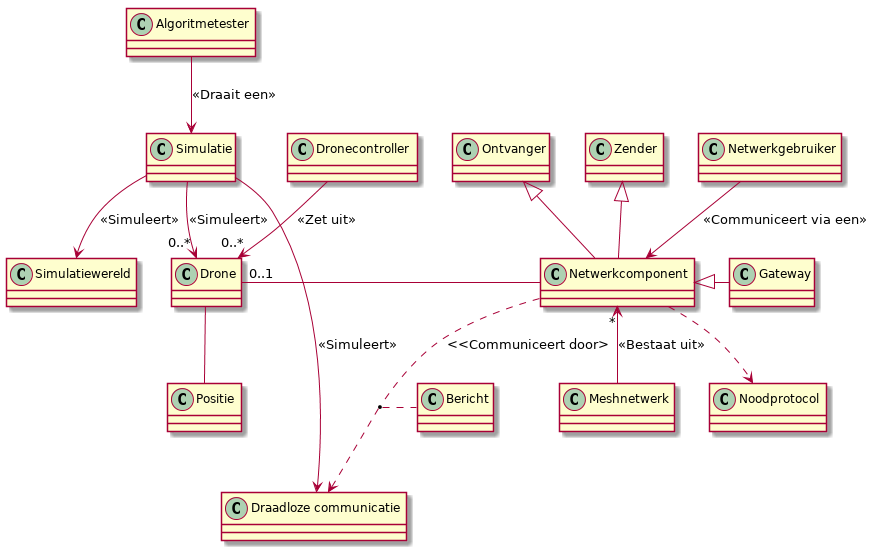
\includegraphics[width=\linewidth]{UML/out/DomeinModel/DomeinModel/DomeinModel.png}\end{center}
	\caption{Domeinmodel}
	\label{fig:toplogienetwerkuml}
\end{figure}

\chapter{Use-case omschrijvingen}
\label{Usecase}
\section{Use case}
\label{Usecase:1}
\subsection{Fully-dressed use case description}
\label{Usecase:1:fully-dressed}
\subsection{System Sequence Diagram (optional)}
\label{Usecase:1:systemsequence}
\subsection{Operation Contracts (optional)}
\label{Usecase:1:fully-operation}
\section{Use case 2 ( and so on)}
\label{Usecase:2}
\subsection{Fully-dressed use case description}
\label{Usecase:2:fully-dressed}
\subsection{System Sequence Diagram (optional)}
\label{Usecase:2:systemsequence}
\subsection{Operation Contracts (optional)}
\label{Usecase:2:fully-operation}
\section{Use case 2 ( and so on)}


\chapter{Other functional requirements (optional)}
\chapter{Non-functional Requirements}
\section{Performance Efficiency}
\section{Security}
\section{Reliability (and so on)}



\bibliographystyle{apacite}
\bibliography{bilbliography.bib}

\clearpage
\appendix
\chapter{Appendix 1}
\label{app:iteratieplan}





\end{document}